%! Author = zhenxiang
%! Date = 23-3-26

\PassOptionsToPackage{quiet}{xeCJK}  % 抑制无意义的警告
% Preamble
\documentclass[11pt]{ctexart}


% Packages
\usepackage{amsmath}
% graphicx
\usepackage{graphicx}
% 页面设置
\usepackage{geometry}
\geometry{left=2.5cm, right=2.5cm, top=2.5cm, bottom=2.5cm}
% codes
\usepackage{listings}
\usepackage{xcolor}
\usepackage{color}
\definecolor{mygreen}{rgb}{0,0.6,0}
\definecolor{mygray}{rgb}{0.5,0.5,0.5}
\definecolor{mymauve}{rgb}{0.58,0,0.82}
\lstset{ %
	backgroundcolor=\color{white},   % choose the background color; you must add \usepackage{color} or \usepackage{xcolor}
	basicstyle=\ttfamily,            % the size of the fonts that are used for the code
	breakatwhitespace=false,         % sets if automatic breaks should only happen at whitespace
	breaklines=true,                 % sets automatic line breaking
	captionpos=b,                    % sets the caption-position to bottom
	commentstyle=\ttfamily\color{mygreen},    
	% comment style
	deletekeywords={},               % if you want to delete keywords from the given language
	escapeinside={},                 % if you want to add LaTeX within your code
	extendedchars=true,              % lets you use non-ASCII characters; for 8-bits encodings only, does not work with UTF-8
	frame=single,                    % adds a frame around the code
	keepspaces=true,                 % keeps spaces in text, useful for keeping indentation of code (possibly needs columns=flexible)
	keywordstyle=\color{blue},       % keyword style
	language=C++,                    % the language of the code
	morekeywords={},                 % if you want to add more keywords to the set
	numbers=left,                    % where to put the line-numbers; possible values are (none, left, right)
	numbersep=5pt,                   % how far the line-numbers are from the code
	numberstyle=\tiny\color{mygray}, % the style that is used for the line-numbers
	rulecolor=\color{black},         % if not set, the frame-color may be changed on line-breaks within not-black text (e.g. comments (green here))
	showspaces=false,                % show spaces everywhere adding particular underscores; it overrides 'showstringspaces'
	showstringspaces=false,          % underline spaces within strings only
	showtabs=false,                  % show tabs within strings adding particular underscores
	stepnumber=1,                    % the step between two line-numbers. If it's 1, each line will be numbered
	stringstyle=\color{mymauve},     % string literal style
	tabsize=2,                       % sets default tabsize to 2 spaces
	title=\lstname                   % show the filename of files included with \lstinputlisting; also try caption instead of title
}

% Document
\begin{document}

\section{lecture 3 Kernel-Based
	Data Parallel Execution Model}

\newpage
\section{Programming Massively Parallel Processors: Scalable parallel execution}

\subsection{CUDA THREAD ORGANIZATION}

In this chapter, we will study important concepts involved in the control of parallel execution. We will start by learning how thread index and block index can facilitate processing multidimensional arrays. Subsequently, we will explore the concept of flexible resource assignment and the concept of occupancy. We will then advance into thread scheduling, latency tolerance, and synchronization. A CUDA programmer who masters these concepts is
well-equipped to write and understand high-performance parallel applications.


\begin{lstlisting}
	// a 1D grid that consists of 32 blocks, each of which consists of 128 threads. The total number of threads in the grid is 128*32 = 4096.
	dim3 dimGrid(32, 1, 1);
	dim3 dimBlock(128, 1, 1);
	vecAddKernel<<<dimGrid, dimBlock>>>(…);
	//  the following statements accomplish the same as the statements above
	dim3 dog(32, 1, 1);
	dim3 cat(128, 1, 1);
	vecAddKernel<<<dog, cat>>>(…);
	// The grid and block dimensions can also be calculated from other variables.
	dim3 dimGrid(ceil(n/256.0), 1, 1);
	dim3 dimBlock(256, 1, 1);
	vecAddKernel<<<dimGrid, dimBlock>>>(…);
	
	
	//For convenience, CUDA C provides a special shortcut for launching a kernel with one-dimensional grids and blocks. Instead of dim3 variables, arithmetic expressions can be used to specify the configuration of 1D grids and blocks. 
	vecAddKernel<<<ceil(n/256.0), 256>>>(…);
\end{lstlisting}

Unlike the dim3 variables in  the host code, the name of these variables within the kernel functions are part of the CUDA C specification and cannot be changed --i.e., gridDim and blockDim in a kernel always reflect the dimensions of the grid and the blocks.

In CUDA C, the allowed values of gridDim.x, gridDim.y and  gridDim.z range from 1 to 65536. All threads in a block share the same blockid.x, blockidx.y, blockidx.z values.

Among blocks, the blockIdx.x value ranges from 0 to gridDim.x-1 , the blockIdx.y value from 0 to gridDim.y-1 , and the blockIdx.z
value from 0 to gridDim.z-1 .

The total size of a block is limited to 1024 threads, with flexibility in distributing
these elements into the three dimensions as long as the total number of threads does
not exceed 1024. For instance, blockDim(512, 1, 1) , blockDim(8, 16, 4), and
blockDim(32, 16, 2) are allowable blockDim values, but blockDim(32, 32, 2) is
not allowable because the total number of threads would exceed 1024.

The grid can have higher dimensionality than its blocks and vice versa. For
instance, code shows a small toy grid example of gridDim(2, 2, 1) with blockDim(4, 2, 2) . The grid can be generated with the following host code: 

\begin{lstlisting}
	dim3 dimGrid(2, 2, 1);
	dim3 dimBlock(4, 2, 2);
	KernelFunction<<<dimGrid, dimBlock>>>(…);
\end{lstlisting}

块 (1,0) 具有 blockIdx.y =1 和 blockIdx.x =0。这些标签的顺序是最高维度优先的。请注意,这种块标签符号是在设置配置参数的 C 语句中使用的符号顺序的反向顺序。在访问多维数据时,这种反向排序的块标记符号更有效。

% 图片置于当前位置
\begin{figure}[ht]
	\centering
	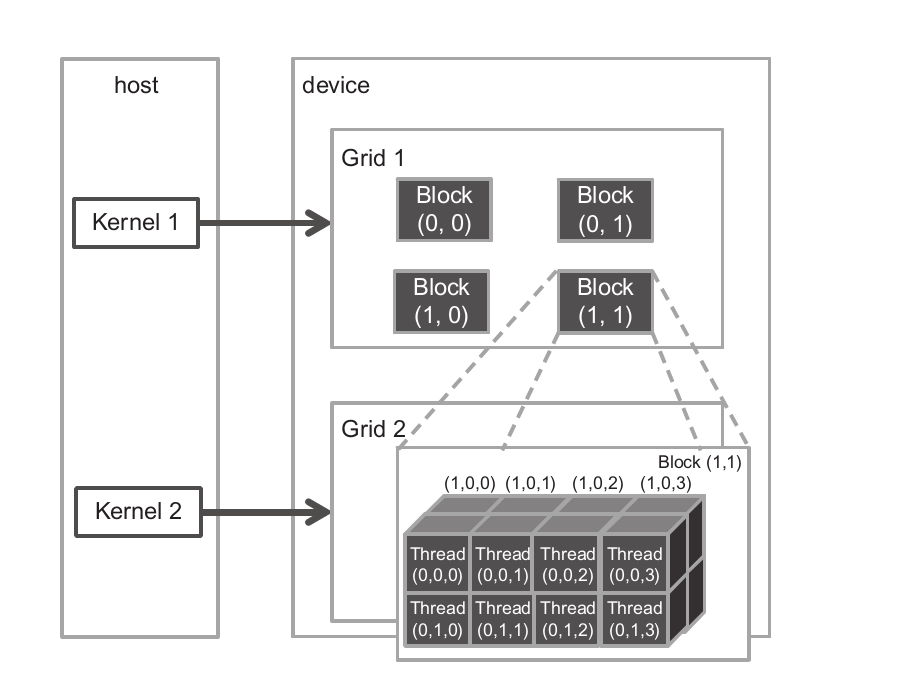
\includegraphics[width=1.0\textwidth]{photos/AmultidimensionalexampleofCUDAgridorganization.png}
	\caption{A multidimensional example of CUDA grid organization}
	\label{fig:1}
\end{figure}




每个 threadIdx 也由三个字段组成:x 坐标 threadId.x,y 坐标 threadIdx.y 和 z 坐标 threadIdx.z。图 3.1 展示了块内线程的组织方式。在此示例中,每个块组织成一个 4 × 2 × 2 的线程数组。所有网格中的块都具有相同的维度;因此,我们只需要显示其中一个。图 3.1 展开了块 (1,1),以显示其 16 个线程。例如,Thread(1,0,2) 具有 threadIdx.z=1、threadIdx.y=0 和 threadIdx.x=2。

Q:为什么这些标签的顺序是最高维度优先的?

A:在CUDA中,blockDim和gridDim参数是以最低维度优先的顺序定义的,这是因为在C语言中,多维数组的元素存储顺序也是以最低维度优先的顺序排列的。例如,对于一个二维数组A[i][j],内存中的数据排列顺序是按照j方向的索引连续存放的,即A[0][0]、A[0][1]、A[0][2]... A[1][0]、A[1][1]、A[1][2]... 以此类推。因此,在C语言中以最低维度优先的顺序定义数组和数据结构可以提高内存访问的效率。

然而,在CUDA中,blockIdx和threadIdx标签的顺序是以最高维度优先的顺序定义的,这是因为这种标签顺序更适合访问多维数组和其他多维数据结构。在CUDA中,每个线程都需要访问多维数组的一个元素,线程的坐标需要映射到数组的下标,因此使用最高维度优先的顺序可以简化这个映射过程,提高内存访问的效率。

使用最高维度优先的顺序可以简化映射过程,提高内存访问的效率,因为它与内存布局的方式是一致的。在计算机内存中,数据通常是按照一维数组的形式存储的,这意味着访问数组中的元素需要知道其索引在内存中的位置,索引的计算涉及到对内存地址的计算和寻址。按照最高维度优先的顺序标记块和线程可以让我们使用相同的索引计算方式来访问多维数据,这种方式可以减少计算量和寻址时间。

例如,假设我们要访问一个二维数组A[i][j],其中i表示行数,j表示列数。按照最高维度优先的顺序,我们可以将其表示为A[i * N + j],其中N表示数组中的列数。这样,我们可以使用相同的方式来访问一维数组和多维数组,并且不需要为每个数组定义一个不同的索引计算公式。

在CUDA程序中,我们通常需要在GPU内存中访问多维数组,按照最高维度优先的顺序标记块和线程可以简化对多维数组的索引计算,从而提高内存访问的效率。这种方法也使得并行程序员更容易处理多维数据,因为它使用了一种常见的编程惯例。

\subsection{MAPPING THREADS TO MULTIDIMENSIONAL DATA}

The choice of 1D, 2D, or 3D thread organizations is usually based on the nature of
the data. Pictures are 2D array of pixels. Using a 2D grid that consists of 2D blocks is
often convenient for processing the pixels in a picture.


Analogously, we should expect that the picture processing kernel function will have if statements to test whether the thread indexes threadIdx.x and threadIdx.y fall within the valid range of pixels.

\begin{lstlisting}
	dim3 dimGrid(ceil(m/16.0), ceil(n/16.0), 1);
	dim3 dimBlock(16, 16, 1);
	colorToGreyscaleConversion<<<dimGrid,dimBlock>>>(d_Pin,d_Pout,m,n);
\end{lstlisting}

\begin{equation}
	L = r * 0.21 + g * 0.72 + b * 0.07
\end{equation}

\begin{lstlisting}
	// we have 3 channels corresponding to RGB
	// The input image is encoded as unsigned characters [0, 255]
	__global__
	void colorToGreyscaleConversion(unsigned char * Pout, unsigned
	char * Pin, int width, int height) {,
		int Col = threadIdx.x + blockIdx.x * blockDim.x;
		int Row = threadIdx.y + blockIdx.y * blockDim.y;
		if (Col < width && Row < height) {
			// get 1D coordinate for the grayscale image
			int greyOffset = Row*width + Col;
			// one can think of the RGB image having
			// CHANNEL times columns than the grayscale image
			int rgbOffset = greyOffset*CHANNELS;
			unsigned char r = Pin[rgbOffset]; // red value for pixel
			unsigned char g = Pin[rgbOffset + 2]; // green value for pixel
			unsigned char b = Pin[rgbOffset + 3]; // blue value for pixel
			// perform the rescaling and store it
			// We multiply by floating point constants
			Pout[grayOffset] = 0.21f*r + 0.71f*g + 0.07f*b;
		}
	}
\end{lstlisting}

\subsection{IMAGE BLUR: A MORE COMPLEX KERNEL}

\begin{lstlisting}
	__global__
	void blurKernel(unsigned char * in, unsigned char * out, int w, int h){
			int Col  = blockIdx.x * blockDim.x + threadIdx.x;
			int Row = blockIdx.y * blockDim.y + threadIdx.y;
			
			if (Col < w && Row < h) {
				int pixVal = 0;
				int pixels = 0;	
				// Get the average of the surrounding BLUR_SIZE x BLUR_SIZE box
				for (int blurRow = - BLUR_SIZE; blurRow < BLUR_SIZE + 1; ++blurRow) {
						int curRow = Row + blurRow;
						int curCol = Col + blurCol;
						// Verify we have a valid image pixel
						if(curRow > -1 && curRow < h && curCol > -1 && curCol < w) {
								pixVal += in[curRow * w + curCol];
								pixels++; // Keep track of number of pixels in the avg	
					}		
			
			}
		}
		// Write our new pixel value out
		out[Row * w + Col] = (unsigned char)(pixVal /pixels); 

	}

}
\end{lstlisting}

\end{document}